\section{Triển khai Lắp ráp Phần cứng}

Sản phẩm được xây dựng dựa trên triết lý thiết kế "Module hóa", cho phép người dùng tùy biến chức năng một cách linh hoạt thông qua việc lắp ghép các khối phần cứng.

\begin{figure}[h]
    \centering
    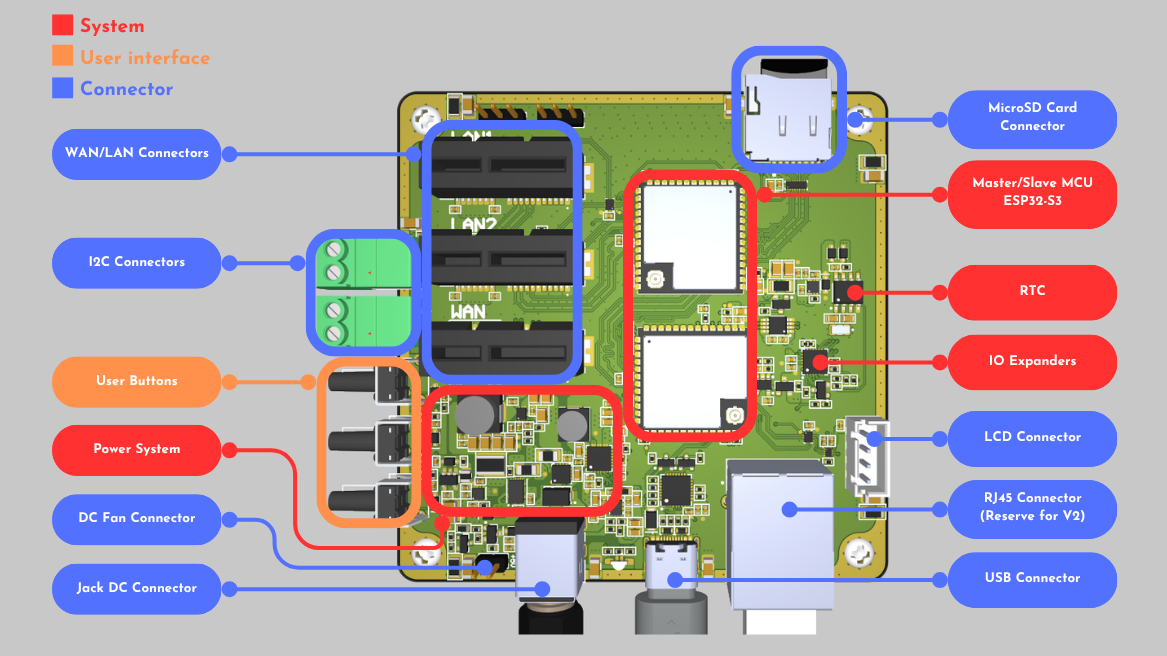
\includegraphics[width=0.9\textwidth]{figures/DATN/Assembly_Diagram_Top.png}
    \caption{Top Assembly Diagram }
\end{figure}
\begin{figure}[h]
    \centering
    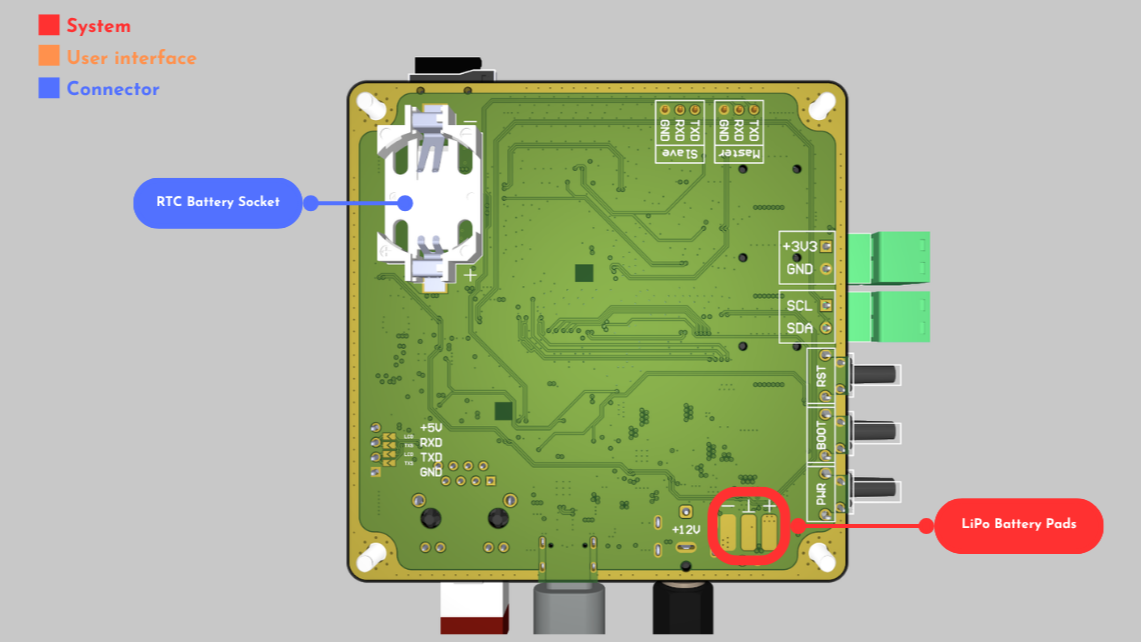
\includegraphics[width=0.9\textwidth]{figures/DATN/Assembly_Diagram_Bottom.png}
    \caption{Bottom Assembly Diagram }
\end{figure}
% \newpage
% \begin{figure}[h]
%     \centering
%     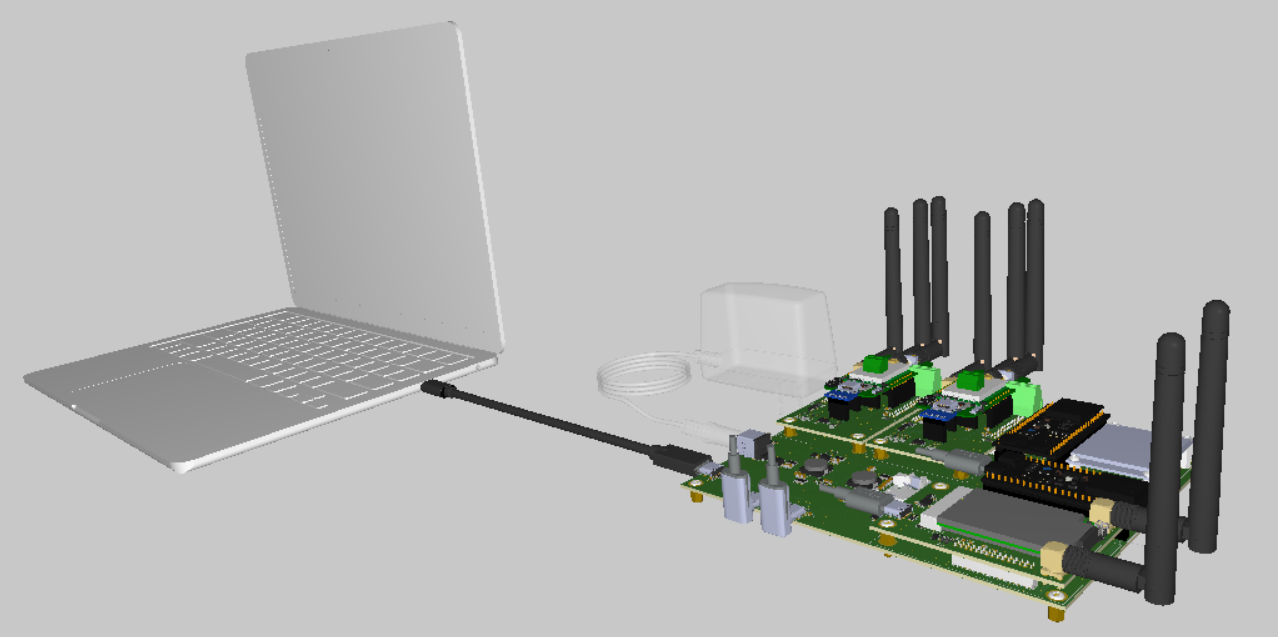
\includegraphics[width=0.8\textwidth]{figures/assembly_3d.png}
%     \caption{Mô hình 3D kết nối thiết bị.}
% \end{figure}

\begin{enumerate}
    \item \textbf{Bo mạch chủ (Baseboard):}
    Bo mạch chủ tích hợp hai vi điều khiển ESP32-S3 (Master và Slave) cùng hệ thống quản lý nguồn tập trung. Hệ thống nguồn cung cấp đồng thời các ray 5V và 3.3V để cấp nguồn cho các module.

    \item \textbf{Cơ chế kết nối Module Adapter:}
    Việc lắp ráp các module chức năng được thông qua các chân cắm \textbf{WAN, LAN1, LAN2 Adapter Connection} đã được định nghĩa sẵn trên Baseboard:
    \begin{itemize}
        \item \textbf{Khe cắm WAN:} Thường lắp ráp các module kết nối mạng không dây như Wi-Fi, LTE 4G hoặc Ethernet.
        \item \textbf{Khe cắm LAN1/LAN2:} Dành cho các module giao tiếp công nghiệp hoặc mạng nội bộ như RS485, LoRaWAN hoặc Zigbee.
    \end{itemize}

    \item \textbf{Programmer USB-C:}
    Cổng USB-C sử dụng cho việc cấu hình IoT Gateway.
\end{enumerate}

\begin{figure}[h]
    \centering
    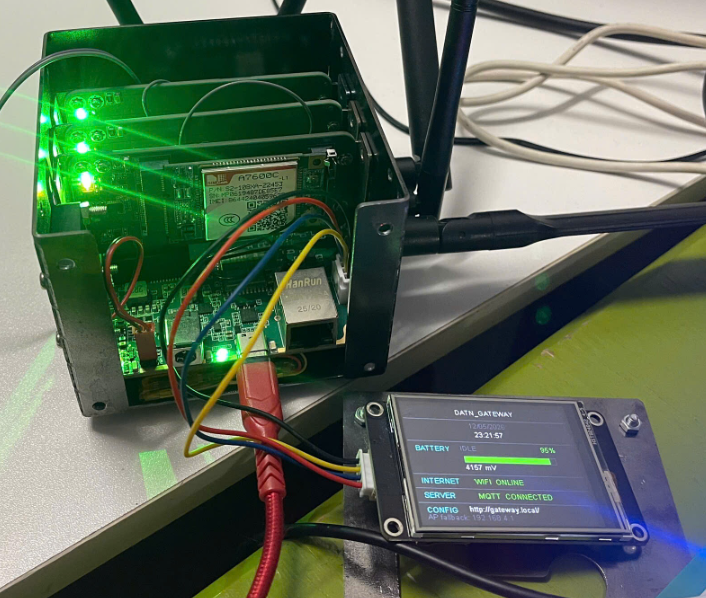
\includegraphics[width=0.75\textwidth, height=9cm, keepaspectratio]{figures/DATN/hinh_anh_thuc_te.png}
    \caption{Hình ảnh sản phẩm thực tế.}
\end{figure}

% \newpage

\begin{figure}[H]
    \centering
    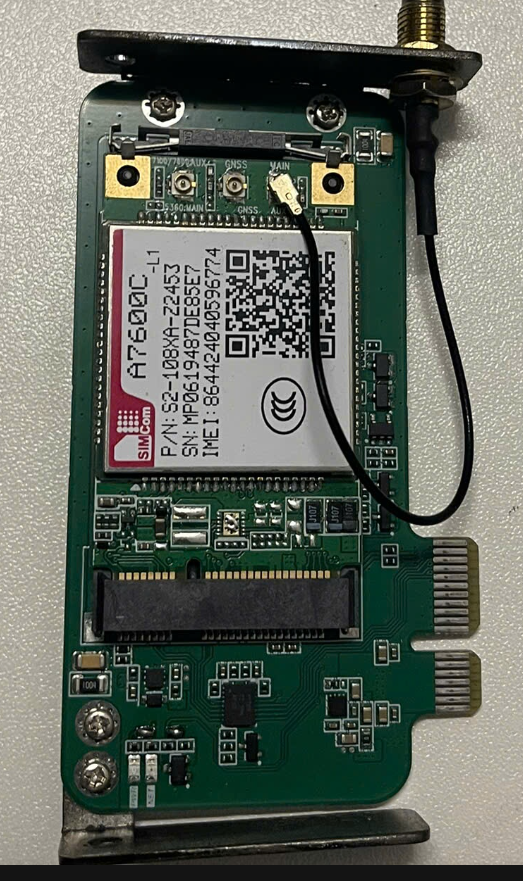
\includegraphics[width=0.4\textwidth, height=6.5cm, keepaspectratio]{figures/DATN/wan_adapter_lte_real.png}
    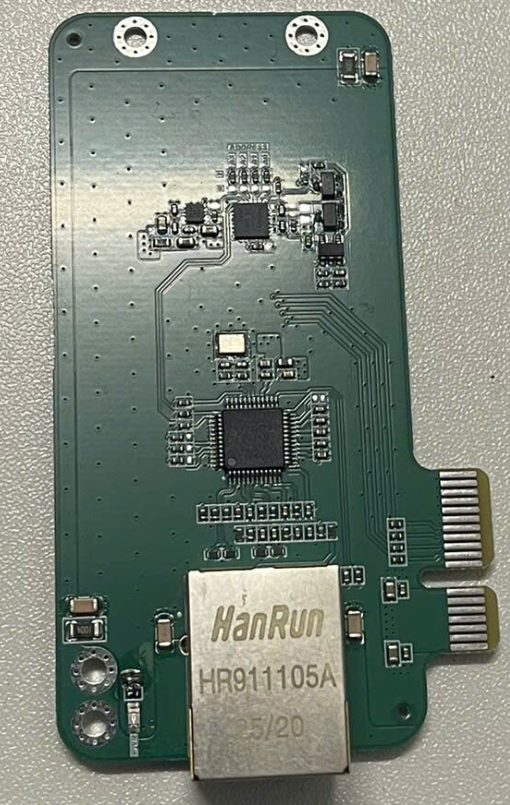
\includegraphics[width=0.4\textwidth, height=6.5cm, keepaspectratio]{figures/DATN/wan_adapter_ethernet_real.png}
    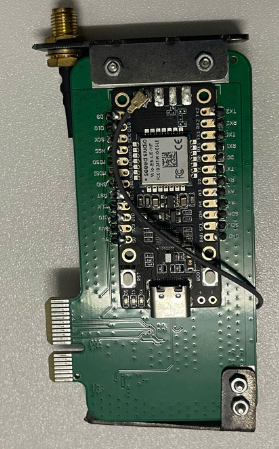
\includegraphics[width=0.4\textwidth, height=6.5cm, keepaspectratio]{figures/DATN/lan_adapter_lorawan_real.png}
    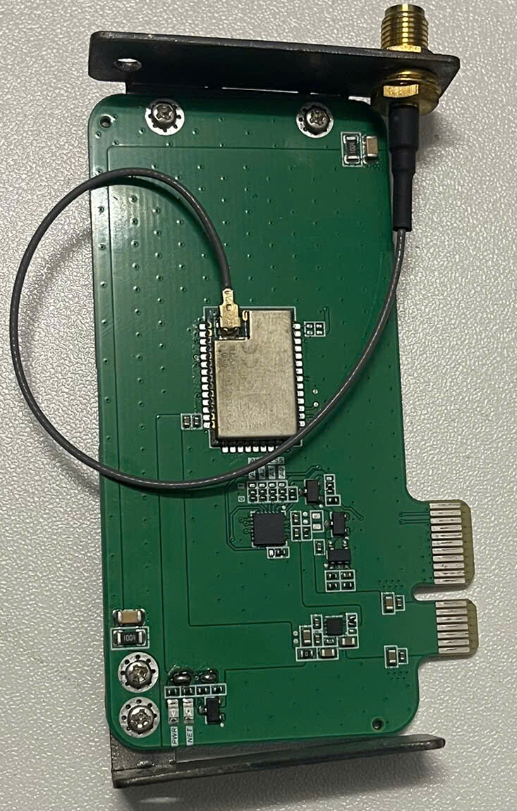
\includegraphics[width=0.4\textwidth, height=6.5cm, keepaspectratio]{figures/DATN/lan_adapter_zigbee_real.png}
    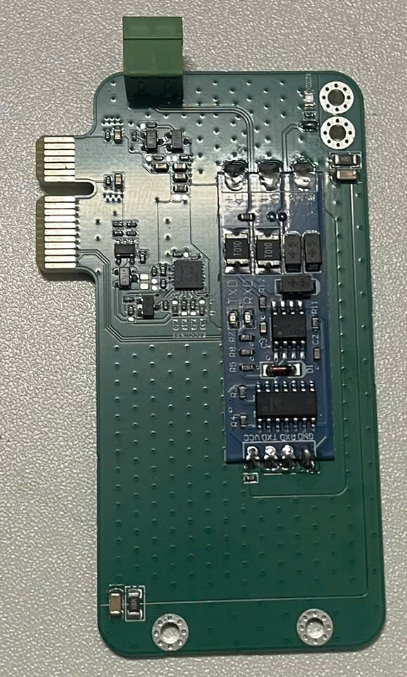
\includegraphics[width=0.4\textwidth, height=6.5cm, keepaspectratio]{figures/DATN/lan_adapter_rs485_real.png}
    \caption{Các Module Adapter đang hỗ trợ.}
\end{figure}

\subsection{Kết quả kết nối thiết bị đầu cuối}

Để kiểm chứng khả năng tích hợp đa giao thức, hệ thống IoT Gateway được triển khai thử nghiệm thực tế cùng với nhiều thiết bị đầu cuối hoạt động đồng thời. Cụ thể, các thiết bị kết nối vào hệ thống bao gồm:

\begin{itemize}
    \item \textbf{BLE (Bluetooth Low Energy):} Các node cảm biến nhiệt độ--độ ẩm (DA2\_SENSOR) và thiết bị LED GATT (DA2\_LED\_GATT) giao tiếp trực tiếp qua BLE Native với LAN-MCU.
    \item \textbf{Zigbee:} Node cảm biến Zigbee (E180-ZG120B, EBYTE) kết nối qua LAN Adapter, dữ liệu được chuyển tiếp lên LAN-MCU qua UART.
    \item \textbf{LoRa P2P:} Node đầu cuối (Wio-E5-LE mini) truyền dữ liệu theo giao thức LoRa Point-to-Point, thu thập qua LAN Adapter.
    \item \textbf{MQTT Broker cục bộ:} Raspberry Pi đóng vai trò server MQTT (Mosquitto), nhận dữ liệu telemetry từ Gateway và cung cấp dashboard giám sát qua ThingsBoard.
\end{itemize}

\begin{figure}[H]
    \centering
    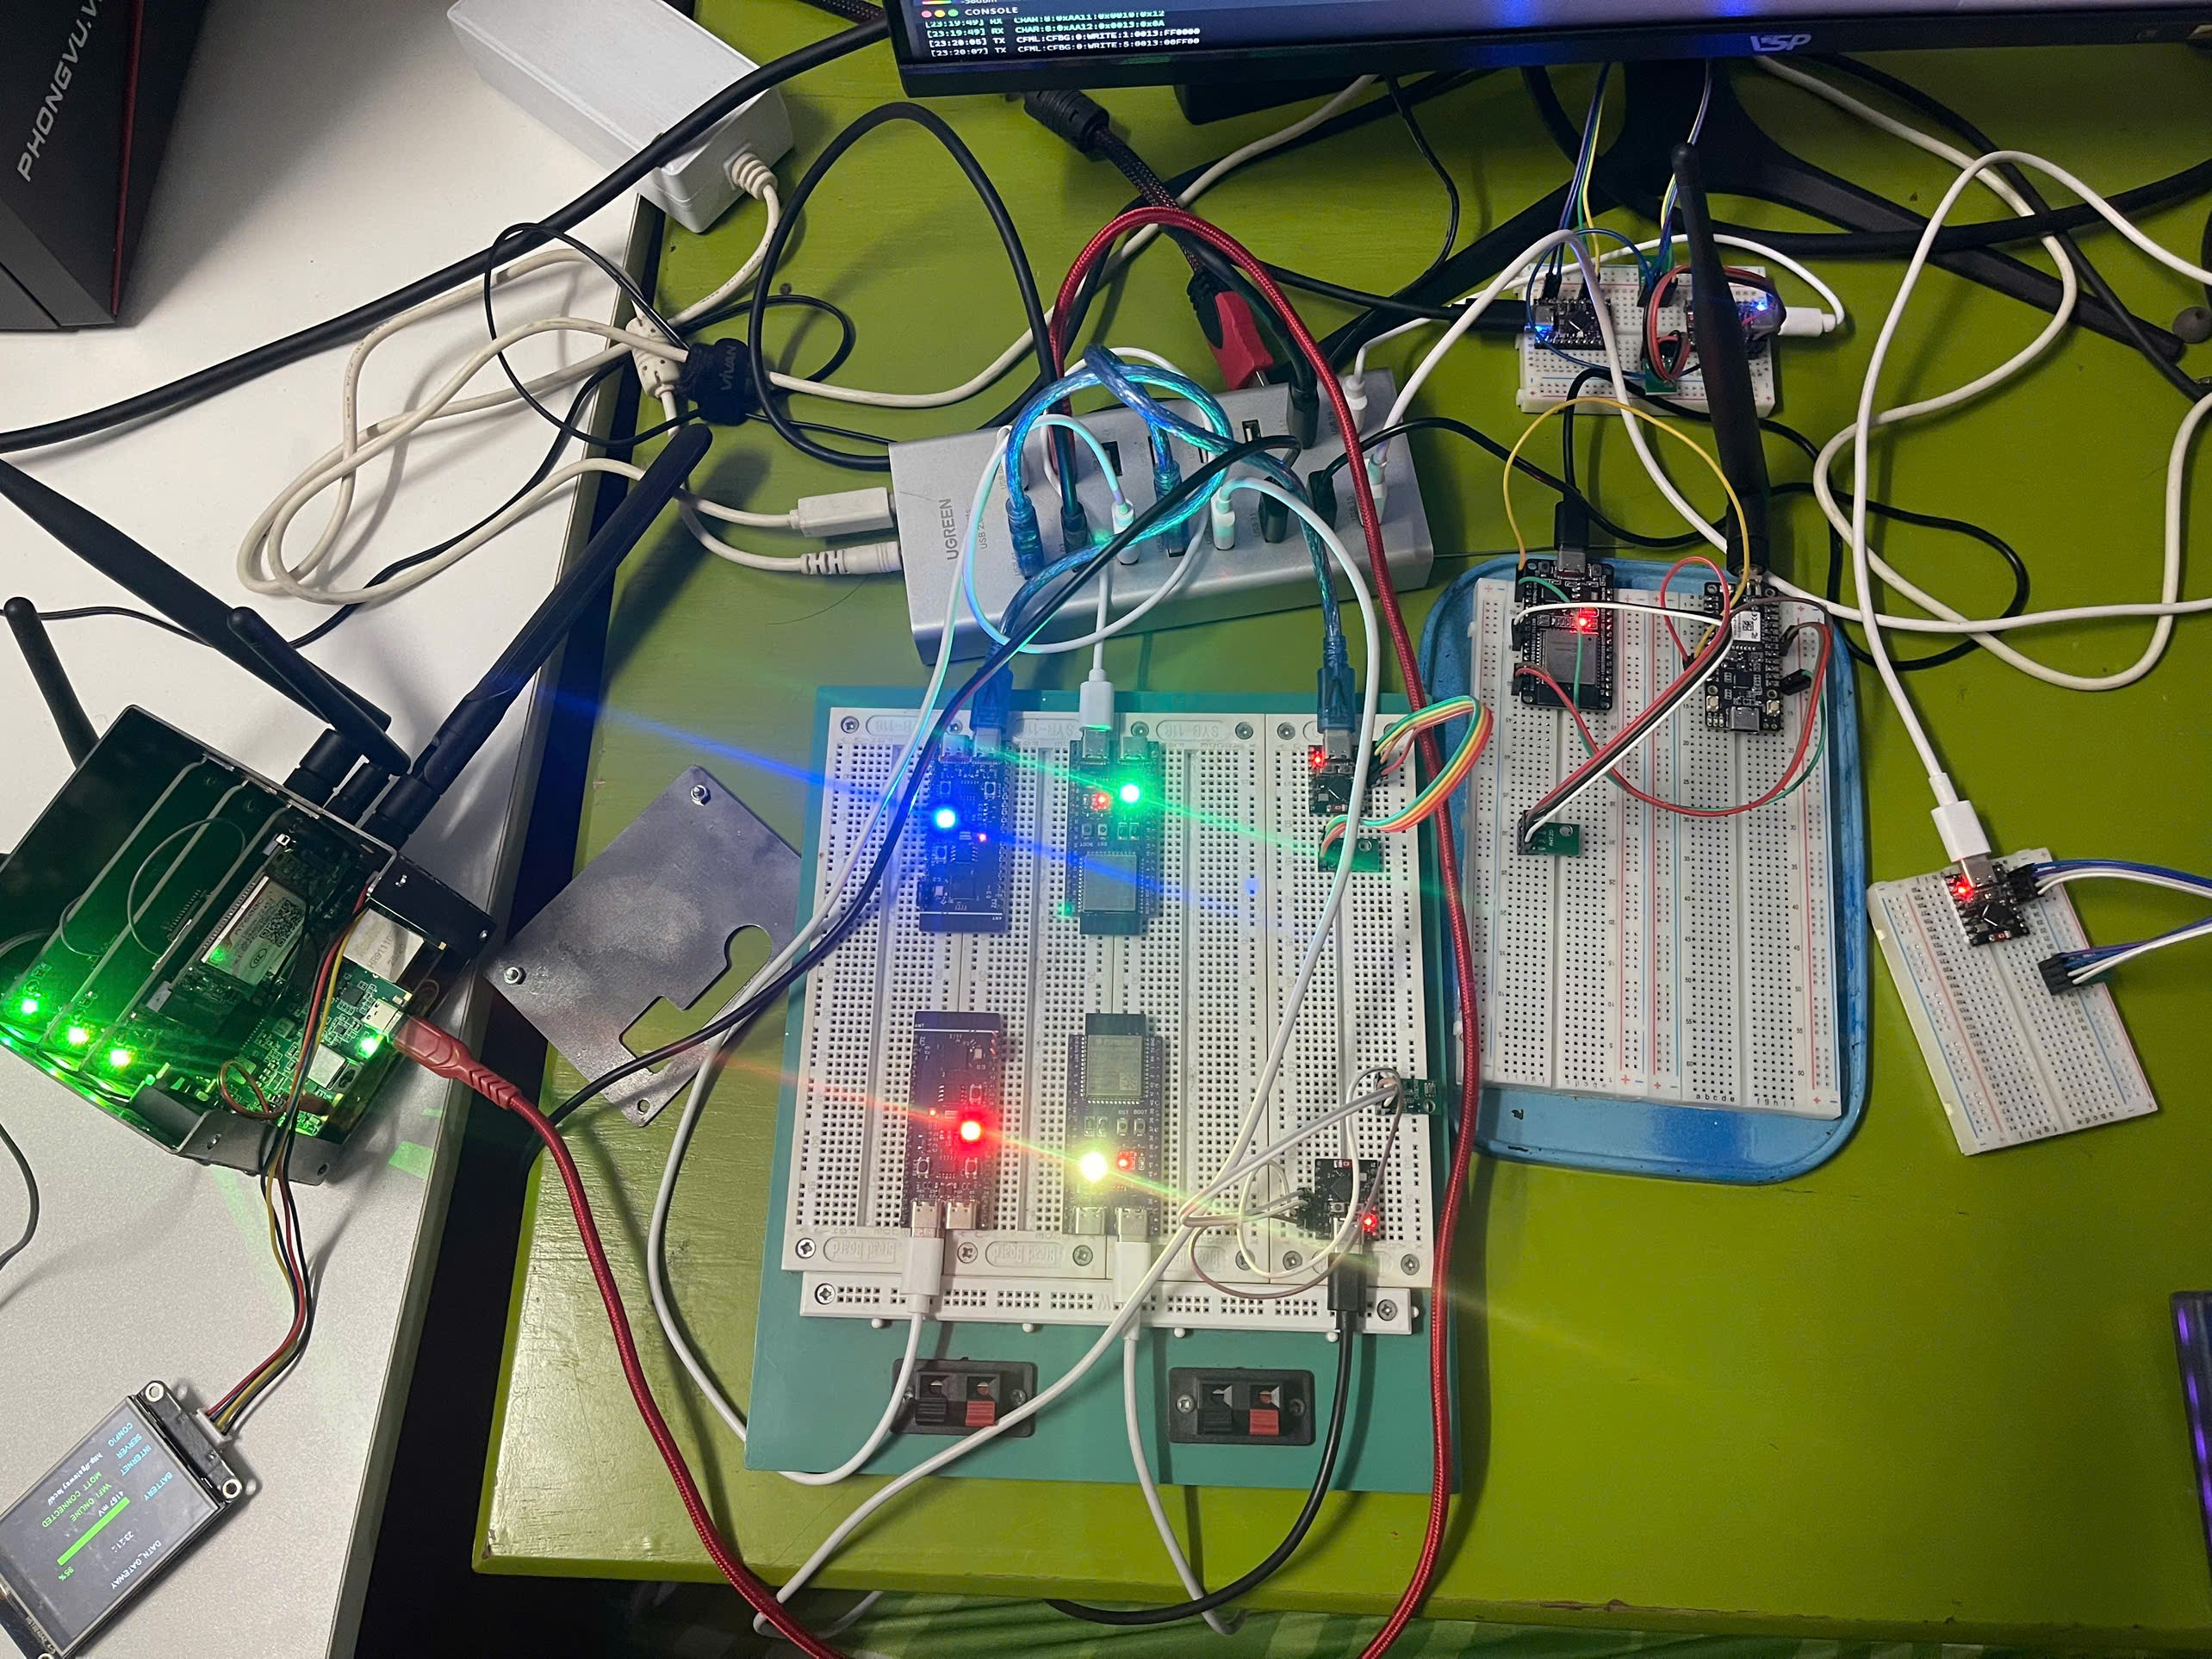
\includegraphics[width=0.9\textwidth]{figures/DATN/trien_khai_ket_noi.png}
    \caption{Prototype IoT Gateway kết nối đồng thời với các thiết bị đầu cuối BLE, Zigbee và LoRa P2P trong môi trường thử nghiệm.}
    \label{fig:trien_khai_ket_noi}
\end{figure}

Kết quả cho thấy gateway nhận diện tự động tất cả module adapter đang cắm (dựa trên Device ID 4-bit từ IO Expander), khởi tải driver tương ứng từ NVS và thiết lập kênh truyền dữ liệu liên tục lên cloud mà không cần can thiệp thủ công vào firmware.
